% Rien d'autre à faire qu'afficher le titre
\begin{frame}
\titlepage 
\end{frame}

\begin{frame}
\frametitle{Какой товар?}
\begin{enumerate}[\Sun]
	\item Товары первого уровня: нефть, газ, золото...
	
	\item Товары второго уровня: аммиак, карбонилы...
	
	\item Усложнение задачи по сравнению с товарами первого уровня (переработка, зависимость от товаров первого уровня, ...)
	
	\item Цен много, что делать? - Использовать базисные цены.
	
	\item Разветвлённая товарная сеть товара второго уровня
	
	\item Общие тренды, следовательно, при прогнозе одного порта можно учитывать другие.
\end{enumerate}
\end{frame}

\begin{frame}
\frametitle{Описание данных}
\begin{table}[]
	\begin{tabular}{|c|c|}
		\hline
		Товар                 & Аммиак         \\ \hline
		Количество "портов"   & 9              \\ \hline
		Тип данных            & Временные ряды \\ \hline
		Периодичность         & Неделя         \\ \hline
		Старт                 & 04.07.2004     \\ \hline
		Финиш                 & 12.01.2020     \\ \hline
		Количество наблюдений & 811            \\ \hline
	\end{tabular}
\end{table}

\end{frame}



\begin{frame}
\frametitle{Примеры рядов}

\begin{center}
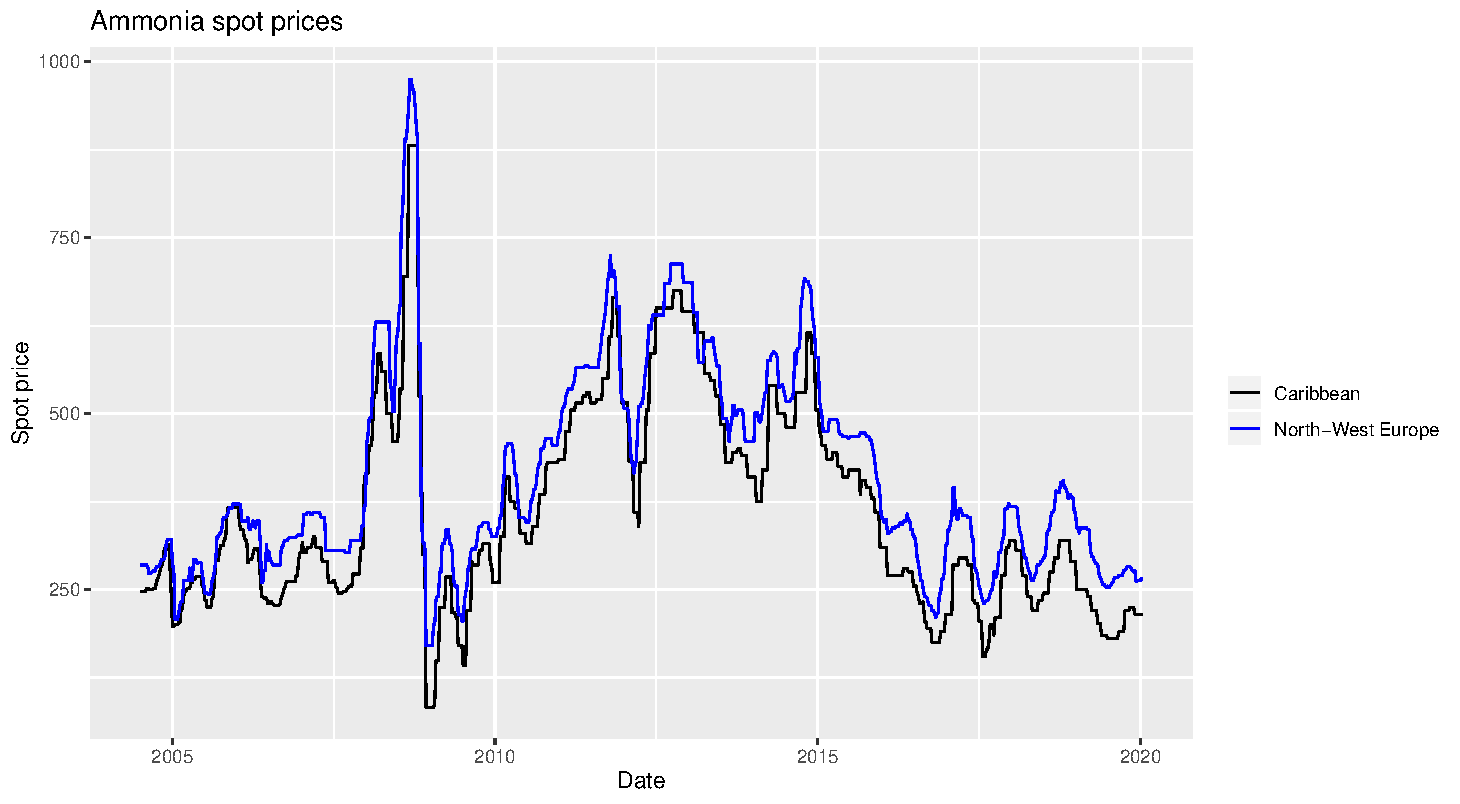
\includegraphics[width = \linewidth]{slides/series.pdf}
\end{center}
\end{frame}

\begin{frame}
\frametitle{Задачи}

\begin{enumerate}[\Sun]
\item Научиться прогнозировать цену в определённом формате на определённый горизонт для каждого порта
\item Протестировать методы и разные подходы, сопоставить точность прогнозов
\item На выходе получить набор некоторых утверждений, позволяющих строить прогноз на каждом порту.
\end{enumerate}
\end{frame}

\begin{frame}
\frametitle{Структура}
\begin{enumerate}
	\item Какой набор экзогенных переменных взять?
	
	\item Какова функциональная форма модели (абсолютные, разности, темпы)?
	
	\item Учёт динамики и глубина прогноза?
	
	$ \hat{y}_i = \alpha y_{i-1} + \beta $ или $ \hat{y}_i = \alpha \hat{y}_{i-1} + \beta $
	
	\item Критерий качества оценки модели?
	
	\item Критерий качества прогноза модели и трактуем ли он?
	
\end{enumerate}
\end{frame}


\begin{frame}
\frametitle{Критерий качества оценки модели}
\begin{enumerate}
	\item Характеристики метрики? BDP, bounded influence function, asympthotic efficiency, reaction to non-normality
	
	\item BDP
	
	\item Ограниченная influence function
	
	\item Реакия на ненормальность остатков
	
	\item Эффективность относительно OLS
	
	\item Реакция на ненормальность остатков
	
	
\end{enumerate}
\end{frame}


